\documentclass[12pt]{article}
\usepackage[a4paper,margin=2.35cm]{geometry}
\usepackage{amsmath,amssymb,amsfonts,bm,booktabs,enumitem,graphicx,microtype,hyperref}
\graphicspath{{figures/}{slides/figures/}{slides/}}
\hypersetup{colorlinks=true,linkcolor=blue,urlcolor=blue}
\setlength{\parskip}{0.72em}
\setlength{\parindent}{0pt}
\setlist[itemize]{topsep=0.2em,itemsep=0.15em}
\setlist[enumerate]{topsep=0.2em,itemsep=0.15em}

% Notation follows the Particle Cosmology lecture notes and Lecture I.
\newcommand{\be}{\begin{eqnarray}}
\newcommand{\non}{\nonumber\\}
\newcommand{\ee}{\end{eqnarray}}
\newcommand{\Hs}{\mathcal H}
\newcommand{\Rs}{\mathcal R}
\newcommand{\bk}{\mathbf k}
\newcommand{\bx}{\mathbf x}
\newcommand{\bn}{\hat{\mathbf n}}
\newcommand{\bv}{\mathbf v}
\newcommand{\dd}{\mathrm d}
\newcommand{\Dl}{D_\ell}
\newcommand{\board}[1]{\begin{center}\fbox{\parbox{0.91\linewidth}{\textbf{Key result.} #1}}\end{center}}
\newcommand{\question}[1]{\begin{center}\fbox{\parbox{0.91\linewidth}{\textbf{Check your understanding.} #1}}\end{center}}

\title{The Cosmic Microwave Background II\\
From primordial fluctuations to angular spectra and real data}
\author{RTG 3186 Kickoff Fall Workshop, Staufen}
\date{29 September--1 October 2026}

\begin{document}
\maketitle

\begin{center}
\fbox{\parbox{0.91\linewidth}{
\textbf{Starting point and goal.}
Lecture I ended with acoustic oscillations of the photon--baryon fluid at last
scattering. Before propagating those fluctuations to the observer, we ask what set
their unusually simple initial conditions. We then project three-dimensional
Fourier modes onto a two-dimensional sky, and derive the angular spectrum $C_\ell$.
We then learn what changes when cosmological parameters are varied and finish by
plotting and fitting the public Planck 2018 temperature data ourselves.}}
\end{center}

% ============================================================
\section{Lecture I recap}

Lecture I established the physical ingredients that will become the initial sources
for today's angular-spectrum calculation. The Friedmann equation fixes the expanding
thermal background. Recombination lowers the free-electron abundance, making the
photon mean free path grow and producing a narrow visibility function around last
scattering. At linear order, perturbations can be decomposed into independently
evolving Fourier modes. Before decoupling, photon pressure and baryon inertia drive
acoustic oscillations in the effective temperature
\be
X\equiv\Theta_0+\Psi
\ee
and in the photon--baryon velocity. Baryon loading shifts the oscillator equilibrium,
gravity drives the motion, and photon diffusion damps sufficiently short wavelengths.
Lecture II asks how these three-dimensional perturbations appear on a two-dimensional
sky and how an experiment measures their statistics.

% ============================================================
\section{Why inflation?}

The motivation here follows the inflation chapter of the Particle Cosmology lecture
notes. It is useful to separate the reasons inflation was originally proposed from
the properties of perturbations that were measured later. The original background
puzzles were the near-flat geometry and the uniform CMB temperature. Detailed CMB
measurements subsequently revealed coherent acoustic phases, approximate scale
invariance, and predominantly adiabatic perturbations. Inflation provides one
dynamical framework for both sets of facts.

\subsection{The flatness problem}
Allowing spatial curvature, the Friedmann equation is
\be
H^2=\frac{8\pi G}{3}\rho-\frac{k}{a^2}.
\ee
The sign convention for the curvature density parameter varies in the literature.
For the present argument only its magnitude matters:
\be
|\Omega_k|\equiv\frac{|k|}{a^2H^2}=\frac{|k|}{(aH)^2}.
\ee
During radiation domination $H^2\propto a^{-4}$, giving
$|\Omega_k|\propto a^2$; during matter domination $H^2\propto a^{-3}$,
giving $|\Omega_k|\propto a$. Curvature therefore grows relative to the dominant
energy density throughout the ordinary decelerating hot-Big-Bang evolution.

Running this evolution backward, the small curvature allowed today requires a much
smaller value in the early Universe. Exact flatness is mathematically possible, but
without a mechanism that drives the Universe toward flatness it is a finely selected
initial condition. Since $|\Omega_k|\propto(aH)^{-2}$, a period during which $aH$
increases instead drives curvature toward zero.

\subsection{The horizon problem}
The comoving particle horizon is the distance light could have travelled since the
beginning of the relevant expansion history,
\be
\chi_H(a)=\int_{a_i}^{a}\frac{d\tilde a}{\tilde a^2H(\tilde a)}.
\ee
In a purely radiation- and matter-dominated history this distance is finite. At last
scattering it is of order a few hundred comoving megaparsecs, whereas the comoving
distance from us to the last-scattering surface is roughly $14$ Gpc. The causal scale
therefore covers only an angular region of order a degree. Many widely separated
regions on the observed CMB sky could not have exchanged signals before
recombination in that history, yet their mean temperatures agree to about one part
in $10^5$.

The problem is not that photons from these regions cannot reach us: they clearly do.
It is that the regions could not communicate with one another early enough to
establish nearly identical thermal conditions. A causal explanation requires a
different earlier expansion history or finely correlated initial conditions.

\subsection{Accelerated expansion addresses both background puzzles}
Inflation is a period of accelerated expansion, so both
\be
\dot a>0,qquad \ddot a>0.
\ee
Since $aH=\dot a$, the general condition for the magnitude of the comoving Hubble
radius to shrink is
\be
\frac{d}{dt}\frac{1}{|aH|}<0
\qquad\Longleftrightarrow\qquad
\dot a\,\ddot a>0.
\ee
This also allows an accelerated contracting branch, with $\dot a<0$ and $\ddot a<0$;
inflation refers specifically to the expanding branch. The comoving Hubble radius
therefore shrinks during inflation. A comoving wavelength can
begin below this scale, cross outside it during inflation, and re-enter when the
comoving Hubble radius grows again during radiation or matter domination. The whole
region visible to us can descend from one much smaller patch with a common causal
past. At the same time, $|\Omega_k|\propto(aH)^{-2}$ is dynamically suppressed.

The Hubble radius and the particle horizon are not identical concepts. The former is
the expansion timescale expressed as a length; the latter is an integrated causal
distance. During the standard decelerating eras they are of the same order. Inflation
changes the lower limit and the expansion history in the particle-horizon integral,
allowing the shared causal past that is absent from an extrapolation of the hot Big
Bang alone.

\begin{figure}[ht]
\centering
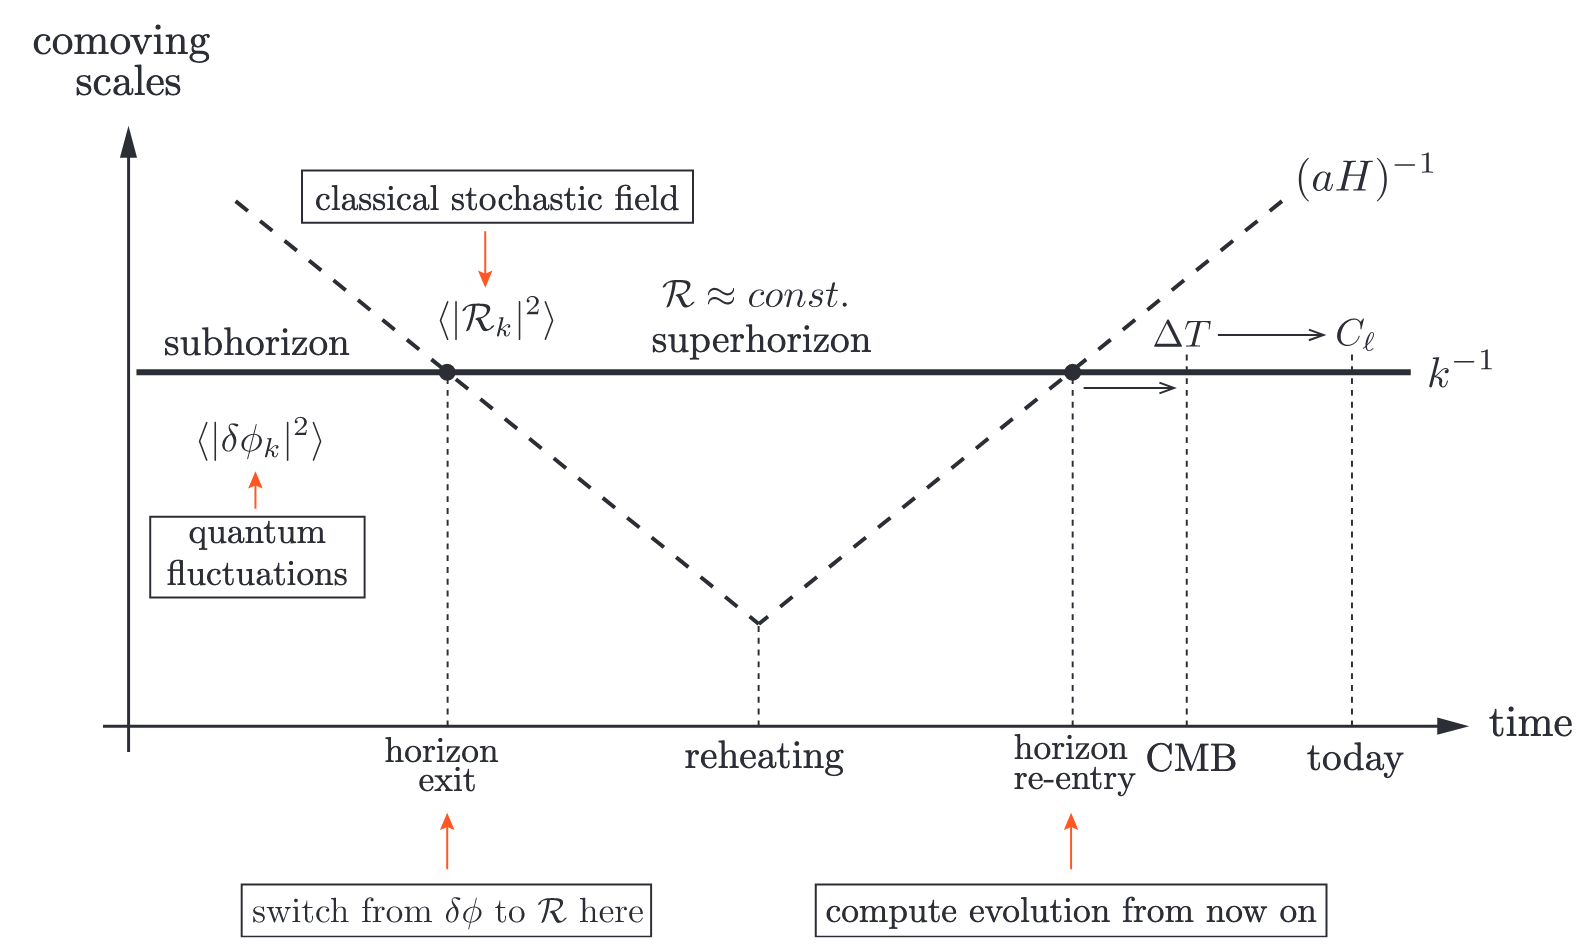
\includegraphics[width=.92\linewidth]{inflation-horizon.png}
\caption{A fixed comoving wavelength begins below the comoving Hubble scale,
exits during inflation, and re-enters during the later decelerating expansion.}
\end{figure}

\subsection{Later CMB evidence concerns the fluctuations}
Lecture I derived acoustic motion mode by mode. The observed sequence of sharp peaks
requires the modes to enter the horizon in a common temporal phase. Random phases
would average the oscillations into a broad, smooth spectrum. The coherence is seen
not only in temperature but also in the relative phases of temperature and
polarization.

The inferred primordial curvature power spectrum is close to scale invariant, and
the perturbations are predominantly adiabatic. The measured spectrum is well
described by
\be
\Delta_{\Rs}^2(k)=A_s\left(\frac{k}{k_0}\right)^{n_s-1},
\qquad n_s\simeq1.
\ee
Thus the power per logarithmic interval varies only slowly with scale. In the simplest
single-field picture, quantum fluctuations begin on subhorizon scales, are stretched
beyond the Hubble radius, and become the classical curvature perturbation $\Rs$. A
single clock also selects adiabatic initial conditions and a common growing mode,
explaining the phase coherence.

We will not derive the quantum generation of $\Rs$ here. For the CMB calculation we
need its statistical spectrum and the fact that subsequent linear evolution is
deterministic for each mode. This is precisely the separation between primordial
statistics and transfer functions used below.

% ============================================================
\section{From last scattering to the observer}

\subsection{What was present at recombination?}
For each Fourier mode $\bk$, Lecture I identified three important quantities at the
last-scattering time $\tau_*$:
\begin{itemize}
\item the photon temperature monopole $\Theta_0=\delta_\gamma/4$;
\item the baryon velocity $\bv_b$, approximately equal to the photon velocity in tight coupling;
\item the metric potentials $\Phi$ and $\Psi$ in conformal Newtonian gauge,
\[
ds^2=a^2(\tau)\left[-(1+2\Psi)d\tau^2+(1-2\Phi)d\bx^2\right].
\]
\end{itemize}
Here $\Theta_0$ denotes the angular monopole of the photon-temperature perturbation
for a Fourier mode. It is unrelated to the symbol $T_0$ for the mean CMB temperature
today.
The photon--baryon density is at an extremum when its velocity is approximately zero,
and vice versa. Density and velocity contributions will therefore appear out of phase.

\subsection{Gravitational and scattering contributions}
For orientation, imagine instantaneous recombination. Integration of the photon
geodesic and the Thomson-scattering source gives the observed fractional temperature
in direction $\bn$,
\be
\boxed{
\Theta(\bn)=
\underbrace{\left[\frac14\delta_\gamma+\Psi\right]_*}_{\text{Sachs--Wolfe}}
-\underbrace{\left.\bn\cdot\bv_b\right|_*}_{\text{Doppler}}
+\underbrace{\int_{\tau_*}^{\tau_0}d\tau\,(\dot\Phi+\dot\Psi)}_{\text{integrated Sachs--Wolfe}}.}
\label{eq:SWDopplerISW}
\ee
Dots denote derivatives with respect to conformal time.

The three pieces have distinct origins:
\begin{enumerate}
\item $\delta_\gamma/4$ is an intrinsic temperature perturbation.
\item $\Psi_*$ gravitationally redshifts a photon climbing out of a potential well.
Together these form the ordinary Sachs--Wolfe contribution.
\item Motion of the last scatterers produces a line-of-sight Doppler shift.
\item If the potentials evolve while a photon travels, it gains or loses additional
energy. This is the integrated Sachs--Wolfe (ISW) effect.
\end{enumerate}
Potentials are nearly constant during matter domination. They evolve near
radiation--matter equality and again when dark energy becomes important. Early ISW
affects the acoustic region; late ISW mainly affects large angular scales.

\subsection{The more accurate line-of-sight solution}
Recombination is not instantaneous. With optical depth $\tilde\tau$ and visibility
$g=-\dot{\tilde\tau}e^{-\tilde\tau}$, all local temperature sources can be collected
in a source function $S_T(k,\tau)$. To connect this notation to
Eq.~\eqref{eq:SWDopplerISW}, write $\chi(\tau)=\tau_0-\tau$. Schematically, projection
into multipoles gives
\be
\Theta_\ell(k)\simeq\int_0^{\tau_0}d\tau\left[
gXj_\ell(k\chi)+gv_bj_\ell'(k\chi)
+e^{-\tilde\tau}(\dot\Phi+\dot\Psi)j_\ell(k\chi)+\cdots\right].
\ee
The first two terms are the finite-width versions of the last-scattering emission and
Doppler terms, while the third is accumulated along the photon path. The ellipsis
includes polarization and other terms in the exact linear treatment; detailed signs
and velocity factors depend on Fourier conventions. Integrating the Doppler term by
parts moves the derivative from $j_\ell$ into its coefficient. All coefficients of
$j_\ell$ can then be packaged in $S_T(k,\tau)$, giving the exact linear form
\be
\boxed{
\Theta_\ell(k)=\int_0^{\tau_0}d\tau\,S_T(k,\tau)
j_\ell[k(\tau_0-\tau)].}
\label{eq:LOS}
\ee
$S_T$ is therefore a compact organization of the visibility-weighted monopole,
potential, velocity, polarization, and ISW terms, rather than a new physical effect.
The spherical Bessel function $j_\ell$ performs the geometric
projection from a Fourier wavelength to an angular multipole. CAMB and CLASS exploit
this line-of-sight organization rather than evolving every photon multipole until today.

\question{Why does one Fourier mode contribute to a range of $\ell$ rather than one
exact $\ell$? Projection through $j_\ell(k\chi)$ has finite width, and real last
scattering also has finite radial width. Nevertheless it is useful to remember
$\ell\sim k\chi_*$.}

% ============================================================
\section{Temperature as a random field on the sky}

\subsection{Why spherical harmonics?}
The CMB temperature is a scalar field on a sphere. The analogue of a Fourier expansion
is a spherical-harmonic expansion,
\be
\boxed{\Theta(\bn)=\sum_{\ell=0}^{\infty}\sum_{m=-\ell}^{\ell}
a_{\ell m}Y_{\ell m}(\bn),}
\label{eq:almexpansion}
\ee
with inverse
\be
a_{\ell m}=\int d\Omega_{\bn}\,Y^*_{\ell m}(\bn)\Theta(\bn).
\ee
The integers have a geometric meaning:
\begin{itemize}
\item $\ell=0$ is the monopole, the mean CMB temperature;
\item $\ell=1$ is the dipole, dominated by our peculiar velocity;
\item increasing $\ell$ describes progressively smaller angular structure, roughly
$\theta\sim\pi/\ell$;
\item for every $\ell$ there are $2\ell+1$ values of $m$.
\end{itemize}

\subsection{Statistical isotropy and the angular spectrum}
We have only one CMB sky, but theoretical initial conditions are stochastic. Angular
brackets denote an ensemble average over hypothetical realizations with the same
cosmological parameters. Statistical isotropy says that no orientation is preferred.
It implies
\be
\boxed{
\langle a_{\ell m}a^*_{\ell' m'}\rangle
=C_\ell\delta_{\ell\ell'}\delta_{mm'}.}
\label{eq:CellDefinition}
\ee
Thus all $2\ell+1$ modes at fixed $\ell$ have the same variance. For a statistically
isotropic Gaussian field, the set of $C_\ell$ contains all two-point information.

The real-space angular correlation function is
\be
\langle\Theta(\bn)\Theta(\bn')\rangle
=\sum_\ell\frac{2\ell+1}{4\pi}C_\ell
P_\ell(\bn\cdot\bn').
\label{eq:angularcorrelation}
\ee
This follows from the addition theorem
\[
\sum_mY_{\ell m}(\bn)Y^*_{\ell m}(\bn')
=\frac{2\ell+1}{4\pi}P_\ell(\bn\cdot\bn').
\]

\subsection{Estimating the spectrum from one sky}
On a complete, noiseless sky an unbiased estimator is
\be
\boxed{\widehat C_\ell=\frac{1}{2\ell+1}
\sum_{m=-\ell}^{\ell}|a_{\ell m}|^2.}
\label{eq:CellEstimator}
\ee
For Gaussian $a_{\ell m}$,
\be
\boxed{\operatorname{Var}(\widehat C_\ell)
=\frac{2}{2\ell+1}C_\ell^2.}
\label{eq:cosmicvariance}
\ee
This is \emph{cosmic variance}. Even a perfect instrument cannot provide additional
independent $m$ modes on the largest scales. At high $\ell$ there are many modes and
the fractional uncertainty becomes smaller.

Observers usually plot power per logarithmic interval in angular scale,
\be
\boxed{D_\ell\equiv\frac{\ell(\ell+1)}{2\pi}C_\ell.}
\label{eq:Dell}
\ee
The measured $D_\ell^{TT}$ has units of $\mu{\rm K}^2$ when dimensional temperature
fluctuations rather than $\Theta$ are used.
Since $\delta T=T_0\Theta$, the dimensionless and dimensional spectra are related by
\be
\boxed{C_\ell^{TT,\,\mu{\rm K}^2}=T_0^2C_\ell^{\Theta\Theta},}
\ee
provided $T_0$ is expressed in $\mu{\rm K}$. The same conversion applies to
$D_\ell$.

\board{The $a_{\ell m}$ describe our particular sky. The $C_\ell$ are ensemble
variances predicted by a model. We estimate them by averaging over the $2\ell+1$
values of $m$, which is why cosmic variance remains.}

% ============================================================
\section{Deriving the temperature angular spectrum}

We now connect the primordial three-dimensional perturbations to the observed
two-dimensional spectrum, following the notation and derivation in the Particle
Cosmology notes.

\subsection{Separate initial conditions from deterministic evolution}
Linear evolution allows us to factor the temperature contribution of a Fourier mode
into the initial curvature perturbation $\Rs_i(\bk)$ and a transfer function. One may
write
\be
\Theta(\bn)=\sum_\ell i^\ell(2\ell+1)
\int\frac{d^3k}{(2\pi)^3}\,
\Theta_\ell(k)\Rs_i(\bk)P_\ell(\hat{\bk}\cdot\bn).
\label{eq:Thetamultipoles}
\ee
The transfer function $\Theta_\ell(k)$ contains all linear evolution after the initial
conditions: acoustic oscillations, baryon loading, gravitational driving, diffusion,
recombination, Doppler and ISW effects, and projection.

For instantaneous recombination, its schematic form is
\be
\Theta_\ell(k)=\widetilde A(k)j_\ell(k\chi_*)
-\widetilde B(k)j_\ell'(k\chi_*),
\ee
The prime on $j_\ell'$ means differentiation with respect to its complete argument
$k\chi_*$; it is not a conformal-time derivative. Here $\widetilde A$ contains the
monopole, potentials, and ISW contribution per unit
$\Rs_i$, while $\widetilde B$ contains the baryon velocity per unit $\Rs_i$. The full
result is Eq.~\eqref{eq:LOS}.

\subsection{The primordial power spectrum}
Statistical homogeneity and isotropy define
\be
\boxed{
\langle\Rs_i(\bk)\Rs_i(\bk')\rangle
=(2\pi)^3\delta(\bk+\bk')\frac{2\pi^2}{k^3}
\Delta_{\Rs}^2(k).}
\label{eq:primordialPS}
\ee
For the simplest inflationary initial conditions,
\be
\Delta_{\Rs}^2(k)=A_s\left(\frac{k}{k_0}\right)^{n_s-1}.
\ee
$A_s$ fixes the primordial amplitude and $n_s$ its scale dependence.

\subsection{Compute the two-point function}
Insert Eq.~\eqref{eq:Thetamultipoles} twice into
$\langle\Theta(\bn)\Theta(\bn')\rangle$. The delta function in
Eq.~\eqref{eq:primordialPS} removes one momentum integral. The angular integral uses
\be
\int d\hat{\bk}\,P_\ell(\hat{\bk}\cdot\bn)
P_{\ell'}(\hat{\bk}\cdot\bn')
=\frac{4\pi}{2\ell+1}P_\ell(\bn\cdot\bn')\delta_{\ell\ell'}.
\ee
The result is
\be
\langle\Theta(\bn)\Theta(\bn')\rangle
=\sum_\ell\frac{2\ell+1}{4\pi}
\left[4\pi\int d\ln k\,\Theta_\ell^2(k)
\Delta_{\Rs}^2(k)\right]P_\ell(\bn\cdot\bn').
\ee
Comparison with Eq.~\eqref{eq:angularcorrelation} identifies
\be
\boxed{
C_\ell^{TT}=4\pi\int d\ln k\,
\Theta_\ell^2(k)\Delta_{\Rs}^2(k).}
\label{eq:CellMaster}
\ee

For any two linear observables $X,Y\in\{T,E\}$,
\be
C_\ell^{XY}=4\pi\int d\ln k\,
\Theta_\ell^X(k)\Theta_\ell^Y(k)\Delta_{\Rs}^2(k).
\ee

\board{Primordial physics is encoded in $\Delta_{\Rs}^2(k)$. Everything that
happens between the initial conditions and the observed sky is encoded in the transfer
functions $\Theta_\ell^X(k)$. Their convolution is the observable $C_\ell^{XY}$.}

\subsection{A useful large-scale check}
On scales larger than the sound horizon at recombination, the ordinary Sachs--Wolfe
relation gives $\Theta\simeq\Rs/5$. The transfer function is approximately
\be
\Theta_\ell(k)\simeq\frac15j_\ell(k\chi_*).
\ee
For a scale-invariant primordial spectrum, the identity
\[
\int_0^\infty\frac{dk}{k}j_\ell^2(k\chi_*)
=\frac{1}{2\ell(\ell+1)}
\]
implies
\be
\frac{\ell(\ell+1)}{2\pi}C_\ell^{TT}\simeq
\frac{A_s}{25},
\ee
approximately constant. This is the Sachs--Wolfe plateau. Acoustic dynamics breaks
the plateau into peaks at smaller angular scales.

% ============================================================
\section{How to read a CMB spectrum}

\begin{figure}[ht]
\centering
\IfFileExists{figures/CMBTT_Planck.pdf}{
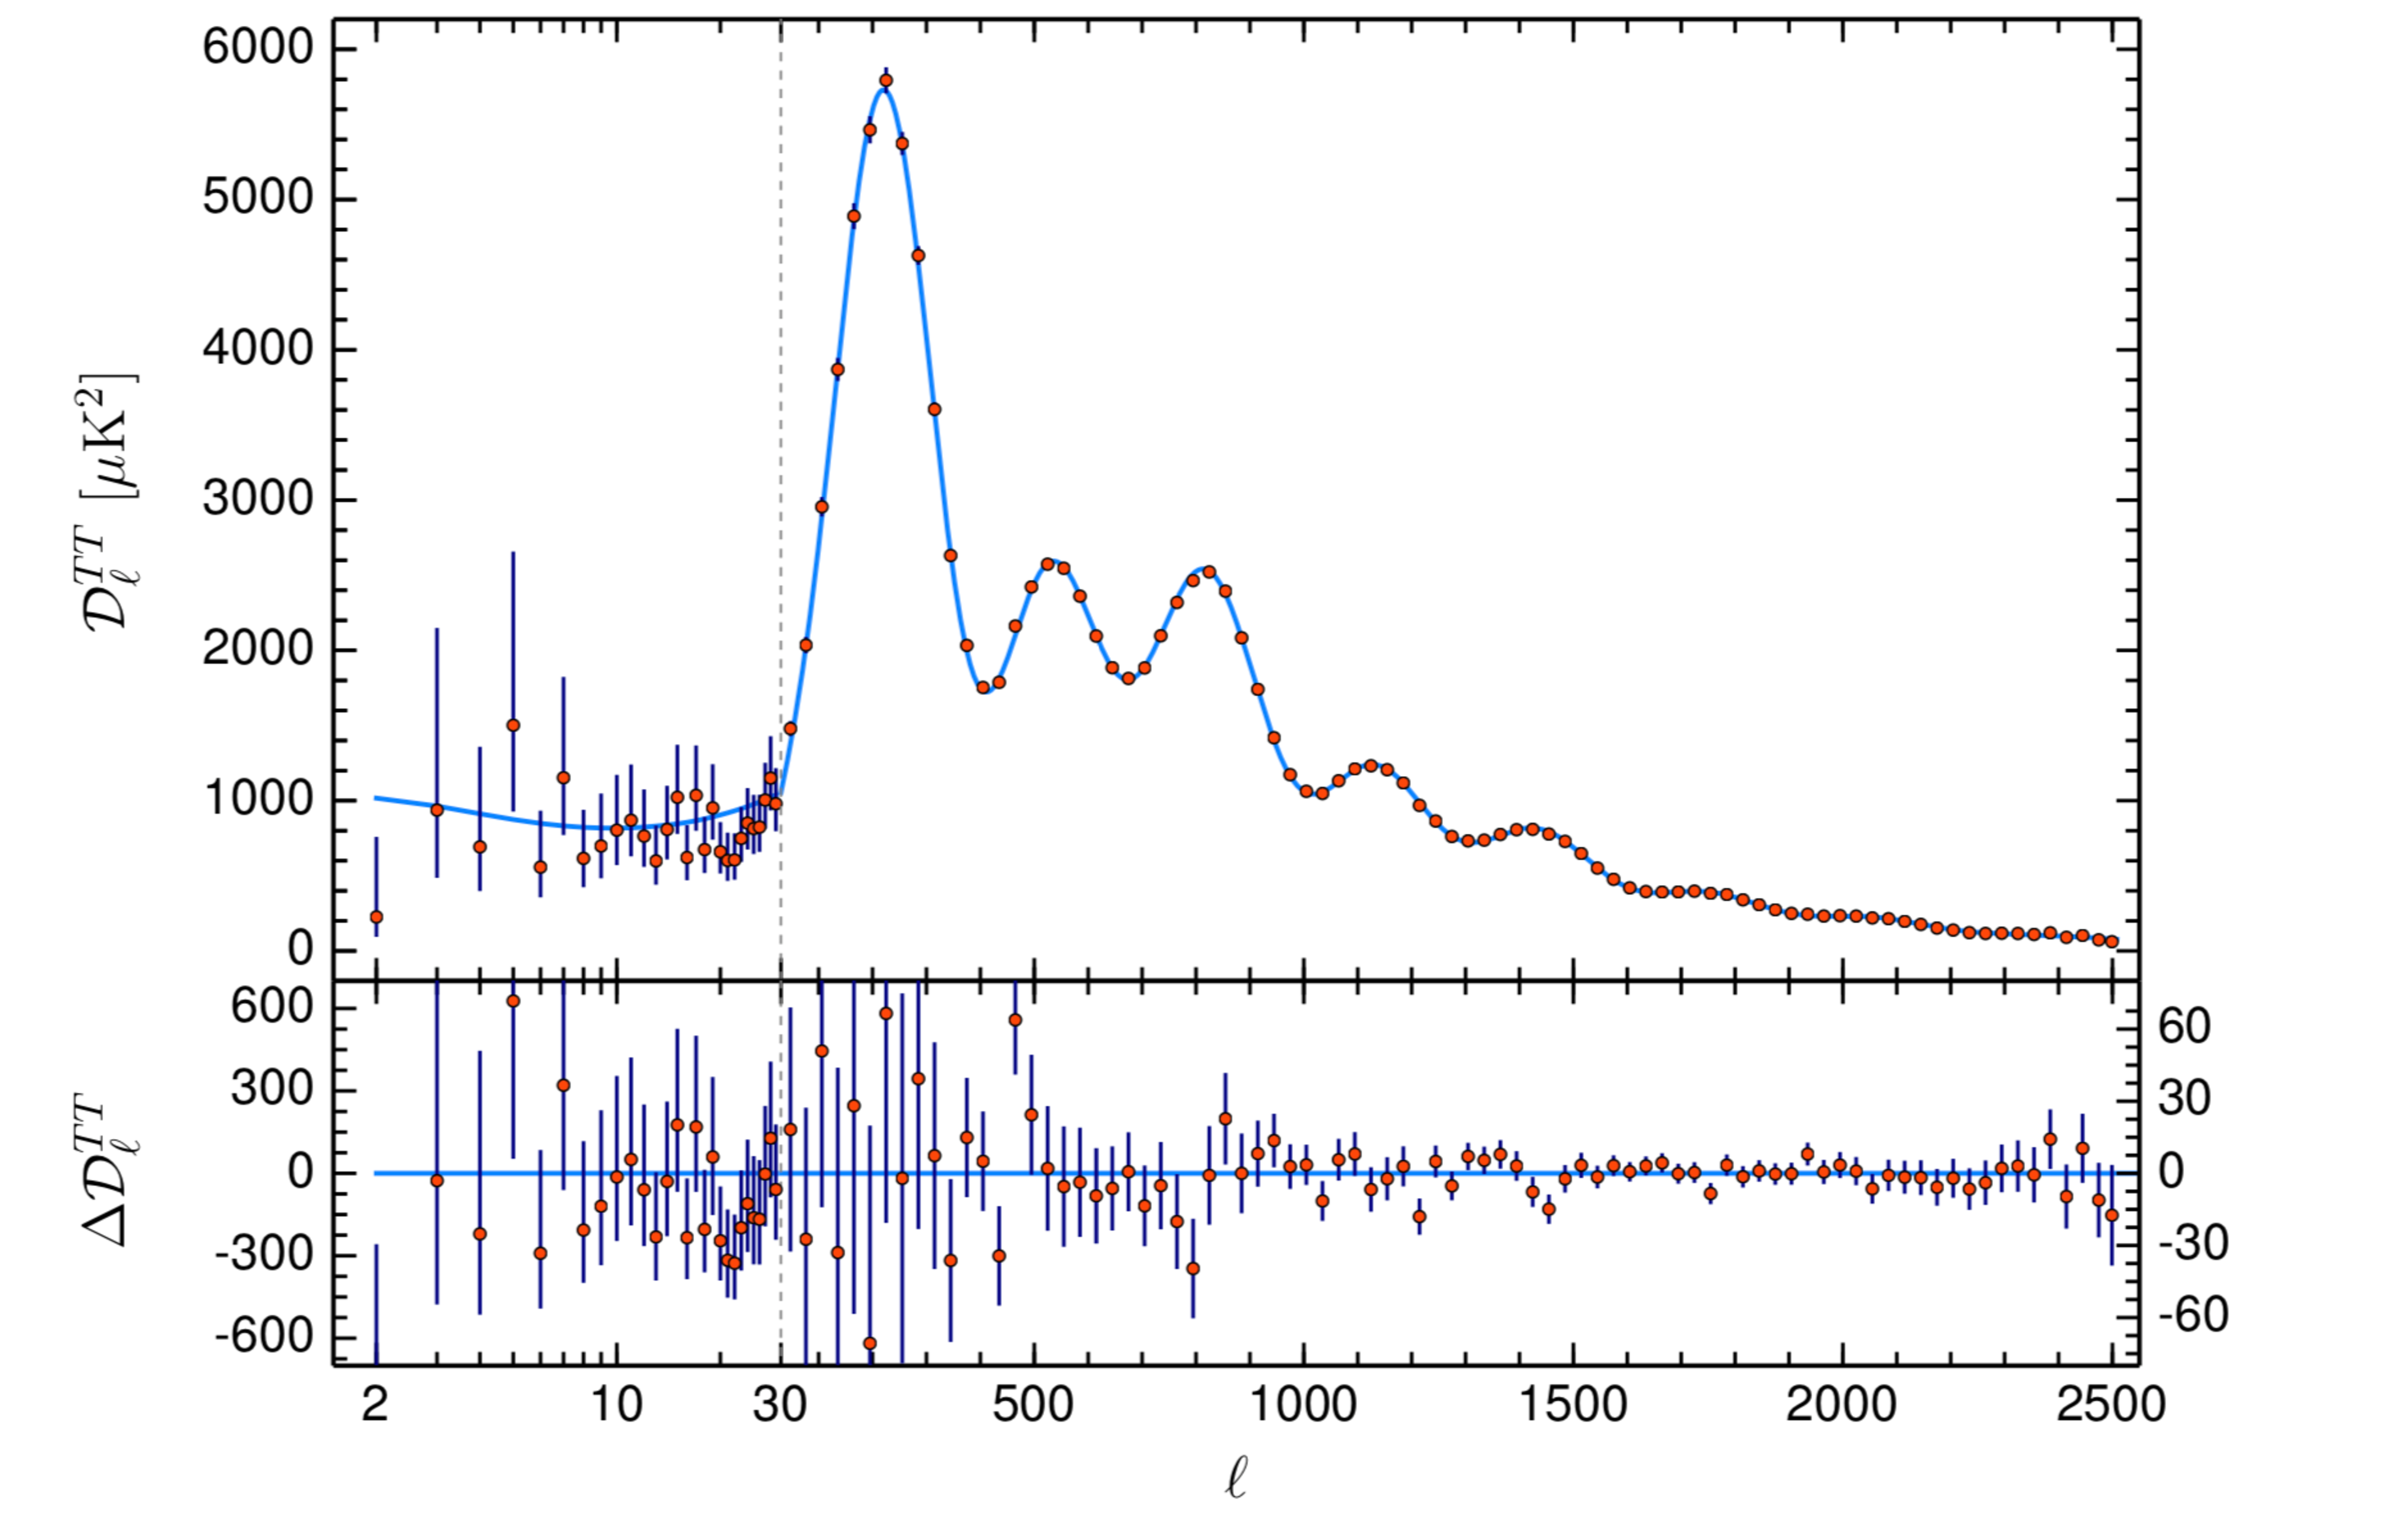
\includegraphics[width=.91\linewidth]{CMBTT_Planck.pdf}}{
\fbox{\parbox[c][4cm][c]{.88\linewidth}{\centering Planck TT spectrum}}}
\caption{Planck temperature bandpowers and a best-fit $\Lambda$CDM spectrum. The
vertical axis is $D_\ell^{TT}=\ell(\ell+1)C_\ell^{TT}/(2\pi)$. Figure retained from
the Particle Cosmology course material, adapted there from Planck 2018.}
\label{fig:PlanckTT}
\end{figure}

The observed spectrum is a compressed history of the Universe:
\begin{itemize}
\item \textbf{Low $\ell$:} ordinary and integrated Sachs--Wolfe effects; cosmic variance is large.
\item \textbf{Acoustic region:} coherent photon--baryon oscillations and gravitational driving.
\item \textbf{High $\ell$:} photon diffusion, finite recombination width, lensing, and foregrounds.
\end{itemize}

The six parameters of minimal flat $\Lambda$CDM are commonly chosen as
\be
\{\omega_b,\,\omega_c,\,\theta_s,\,\tau_{\rm reio},\,A_s,\,n_s\},
\ee
where $\omega_i\equiv\Omega_i h^2$ are physical densities.

\begin{center}
\begin{tabular}{@{}p{.20\linewidth}p{.70\linewidth}@{}}\toprule
Change & Main signature, with other parameters held fixed where possible\\ \midrule
$A_s\uparrow$ & Raises primordial power and hence primary TT/TE/EE; also increases lensing.\\
$n_s\uparrow$ & Tilts the spectrum, increasing small-scale power relative to large-scale power around the pivot.\\
$\omega_b\uparrow$ & Adds baryon inertia: odd compression peaks rise relative to even rarefaction peaks; $c_s$ decreases.\\
$\omega_c\uparrow$ & Moves equality earlier and changes potential decay, radiation driving, and the peak envelope.\\
$\theta_s\uparrow$ & Increases the apparent angular sound horizon and moves the acoustic pattern toward lower $\ell$.\\
$\tau_{\rm reio}\uparrow$ & Suppresses primary power at $\ell\gtrsim20$ by $e^{-2\tau_{\rm reio}}$ and creates low-$\ell$ EE power.\\
$N_{\rm eff}\uparrow$ & Speeds pre-recombination expansion, changes $r_s/r_D$, and produces a free-streaming phase shift.\\
$\sum m_\nu\uparrow$ & Changes late-time expansion and suppresses structure growth and CMB lensing.\\ \bottomrule
\end{tabular}
\end{center}

\subsection{Peak positions: a standard ruler}
The characteristic acoustic scale is
\be
\theta_s=\frac{r_s(\tau_*)}{\chi_*},
\qquad \ell_A\simeq\frac{\pi}{\theta_s}.
\ee
Pre-recombination physics predicts $r_s$; the expansion history between us and last
scattering determines $\chi_*$. The CMB measures their ratio extremely precisely.
Different late-time cosmologies can preserve the same ratio, producing the geometric
degeneracy.

\subsection{Peak heights: competing physical effects}
The ratio of odd to even peaks measures baryon loading. The overall envelope measures
potential decay around equality and thus the matter-to-radiation ratio. The damping
tail compares the diffusion scale with the sound horizon and is sensitive to the
expansion rate and recombination microphysics.

No parameter changes exactly one feature. A proper analysis predicts the full set of
spectra for every parameter point and varies foreground and instrumental nuisance
parameters simultaneously.

\subsection{Polarization supplies phase and geometry information}
Thomson scattering generates linear polarization only if the incident radiation has a
quadrupole. A small quadrupole develops as photons begin to free-stream near
recombination and again at reionization. The Stokes fields $Q$ and $U$ combine into
parity-even E and parity-odd B polarization.

Scalar perturbations produce T and E but no primordial B at linear order. The scalar
spectra are therefore TT, TE, and EE. Since velocity is out of phase with density,
E-mode peaks and TE sign changes provide a strong test of coherent acoustic oscillations.
Reionization creates a low-$\ell$ EE bump and allows $\tau_{\rm reio}$ to be separated
from the high-$\ell$ amplitude combination $A_se^{-2\tau_{\rm reio}}$.

Weak gravitational lensing remaps the sky,
\be
X(\bn)\longrightarrow X(\bn+\nabla\phi),
\ee
smooths acoustic peaks, converts E into B, and generates a connected four-point
function from which the lensing potential $\phi$ can be reconstructed.

\question{Why does measuring EE help if TT already has high signal-to-noise? It
observes different source combinations and phases, breaks parameter degeneracies, and
provides powerful consistency tests against foregrounds and instrumental systematics.}

% ============================================================
\section{How a real experiment obtains bandpowers}

The points in Fig.~\ref{fig:PlanckTT} are not obtained by simply transforming one
perfect temperature map. The actual chain contains several inference problems.

\subsection{Time-ordered detector data}
A scanning polarized detector records a timestream that can be written schematically as
\be
d_t=g_t\left[I_p+Q_p\cos(2\gamma_t)+U_p\sin(2\gamma_t)\right]+n_t+s_t.
\ee
The scalar $d_t$ is one detector datum at time-sample index $t$. Pointing selects
$p=p(t)$, and $\gamma_t$ is the detector orientation. $I_p$ is total intensity;
$Q_p$ and $U_p$ describe linear polarization relative to a chosen pair of axes in
that sky pixel. The factor $g_t$ is calibration, $n_t$ is noise, and $s_t$ represents
instrumental systematics.
Beams, time constants, glitches, pointing, gain, and bandpasses must be characterized.

\subsection{Map-making}
In matrix notation,
\be
\mathbf d=\mathbf A\mathbf m+\mathbf n,
\ee
where the boldface data vector stacks all samples,
$\mathbf d=(d_1,\ldots,d_{N_t})^T$. The pointing matrix $\mathbf A$ connects those
samples to the map vector $\mathbf m$, which contains $(I_p,Q_p,U_p)$ for each pixel.
For Gaussian noise covariance $\mathbf N$, the generalized least-squares map is
\be
\widehat{\mathbf m}=(\mathbf A^T\mathbf N^{-1}\mathbf A)^{-1}
\mathbf A^T\mathbf N^{-1}\mathbf d.
\ee
Large experiments solve this iteratively and use data splits and difference maps to
look for residual systematics.

\subsection{Foreground separation}
The sky depends on observing frequency,
\be
m_\nu(\bn)=a_{\rm CMB}(\bn)+\sum_c f_\nu^c(\bm\beta_c,\bn)a_c(\bn)+n_\nu(\bn).
\ee
Galactic synchrotron dominates polarized low frequencies; thermal dust dominates high
frequencies. Temperature also contains free--free and spinning-dust emission, radio
and infrared sources, the cosmic infrared background, and thermal and kinetic
Sunyaev--Zel'dovich signals. Multiple frequency channels are essential because the CMB
has a known blackbody frequency dependence while foregrounds differ.

\subsection{Cut-sky spectrum estimation}
A Galactic and point-source mask destroys exact spherical-harmonic orthogonality and
couples multipoles. A beam suppresses small angular scales, filtering removes modes,
and noise adds power. Schematically,
\be
\langle\widetilde C_\ell\rangle
=\sum_{\ell'}M_{\ell\ell'}B_{\ell'}^2F_{\ell'}C_{\ell'}
+\widetilde N_\ell.
\ee
$M$ is the mask mode-coupling matrix, $B_\ell$ the beam window, and $F_\ell$ the
filter transfer function. Cross-spectra between maps with independent noise avoid the
mean auto-spectrum noise bias. Nearby multipoles are then grouped into bandpowers.

For a quick uncertainty estimate,
\be
\operatorname{Var}(\widehat C_\ell)\simeq
\frac{2}{(2\ell+1)f_{\rm sky}}(C_\ell+N_\ell)^2.
\ee
This is useful intuition, but real bandpower covariance matrices include mode coupling,
nonuniform noise, beam uncertainty, and foreground correlations.

\subsection{Likelihood and parameter posterior}
Finally,
\be
P(\bm\theta,\bm\eta\mid\mathbf d)\propto
\mathcal L[\mathbf d\mid C_\ell(\bm\theta),\bm\eta]
P(\bm\theta)P(\bm\eta),
\ee
where $\bm\theta$ are cosmological parameters and $\bm\eta$ nuisance parameters.
CAMB or CLASS supplies $C_\ell(\bm\theta)$; a sampler explores the posterior. Low
multipoles require non-Gaussian or map-based likelihood treatments, while suitable
high-$\ell$ bandpowers admit accurate approximations.

\board{A published spectrum is a calibrated, foreground-cleaned, beam- and
mask-corrected statistical estimate with a covariance and nuisance model. It is not
the raw squared transform of a picture of the sky.}

% ============================================================
\section{Hands-on: fit the real Planck TT spectrum}

The accompanying notebook is
\begin{center}
\href{https://colab.research.google.com/github/daanmeerburg/RTG_3186_CMB_Lectures/blob/main/Planck_TT_data_analysis.ipynb}{\textbf{Open the Planck TT exercise directly in Google Colab}}.
\end{center}
The repository also contains the downloadable file
\texttt{Planck\_TT\_data\_analysis.ipynb}. No local installation is required when
using the direct Colab link.

The notebook downloads the official Planck 2018 (PR3) binned TT spectrum from the
Planck archive mirror. The table contains
\be
\{\ell_{\rm eff},\,D_\ell^{\rm data},\,\sigma_-,\,\sigma_+,\,
D_\ell^{\rm best\ fit}\}.
\ee
Students first reproduce the familiar plot of the measured acoustic peaks. They then
fit the deliberately simple model
\be
\boxed{
D_\ell^{\rm model}(A,\alpha)=A\,
D_{\alpha\ell}^{\rm template}.}
\label{eq:teachingmodel}
\ee
The two phenomenological parameters isolate two ideas discussed above:
\begin{itemize}
\item $A$ rescales the vertical amplitude, loosely resembling a change in
$A_se^{-2\tau_{\rm reio}}$;
\item $\alpha$ dilates the horizontal multipole axis, loosely resembling a change in
the angular sound scale $\theta_s$.
\end{itemize}
For the classroom fit, asymmetric errors are averaged and treated as independent
Gaussian uncertainties,
\be
\chi^2(A,\alpha)=\sum_b
\frac{[D_b^{\rm data}-D_b^{\rm model}(A,\alpha)]^2}{\sigma_b^2}.
\label{eq:teachingchi2}
\ee
The notebook plots the best fit, normalized residuals, and approximate 68\% and 95\%
contours in the $(A,\alpha)$ plane.

\subsection{What this fit teaches---and what it does not}
It teaches that a model becomes a curve in data space, uncertainties define a
likelihood, parameters can be correlated, residuals diagnose mismatches, and acoustic
positions are measured far more sharply than one might guess by eye.

It is not a cosmological parameter analysis. The public bandpowers have correlated
errors; the low-$\ell$ likelihood is not Gaussian; foreground and calibration
parameters have already entered the published spectrum; and the template was itself
obtained from a Planck best fit. Research inference instead recomputes TT, TE, and EE
with an Einstein--Boltzmann solver and evaluates the official likelihood including its
covariance and nuisance model.

\question{Why should the notebook find $A\simeq1$ and $\alpha\simeq1$? Because the
template was obtained by fitting essentially these data with a much more complete
model. The exercise tests our simplified compression of that comparison.}

% ============================================================
\section{Outlook: current instruments and future information}

For a measured sky fraction $f_{\rm sky}$, the approximate spectrum uncertainty
\be
\sigma(\widehat C_\ell)\simeq
\sqrt{\frac{2}{(2\ell+1)f_{\rm sky}}}\,(C_\ell+N_\ell)
\ee
organizes the experimental outlook. Better sensitivity and angular resolution lower
$N_\ell$ and make additional polarization and small-scale modes useful. More sky
raises the number of independent modes. Once $N_\ell\ll C_\ell$, however, that
spectrum on that sky is cosmic-variance limited.

Modern CMB bolometers can approach the photon-noise floor set by emission from the
sky, atmosphere, and telescope. This photon noise contains both Poisson fluctuations
in the arrival counts and, for thermal radiation, correlations between photon
arrivals. The latter contribution is called wave noise or bunching noise. If detector noises are
approximately independent,
\be
{\rm NET}_{\rm array}\simeq\frac{{\rm NET}_{\rm det}}{\sqrt{N_{\rm det}}},
\qquad {\rm mapping\ speed}\propto N_{\rm det}.
\ee
This is why the long-running sensitivity trend has depended strongly on putting more
background-limited detectors on the sky. Detector yield, atmosphere, correlated
noise, calibration, beams, and observing efficiency limit the ideal scaling.

The connection to mode counting is direct:
\be
N_{\rm modes}=f_{\rm sky}\sum_{\ell=2}^{\ell_{\max}}(2\ell+1)
\simeq f_{\rm sky}\ell_{\max}^2.
\ee
Future constraints improve when lower noise, broader sky coverage, or better control
of systematics and foregrounds makes more of these modes usable. Frequency channels
do not supply independent copies of one CMB mode. Instead, they separate the CMB from
synchrotron, Galactic dust, the cosmic infrared background, and other emission with
different spectra.

\subsection{Complementary experiments}
The Simons Observatory combines a 6-m Large Aperture Telescope for arcminute scales
with Small Aperture Telescopes optimized for degree-scale polarization. Its expanded
programme includes two SO:UK mid-frequency SATs and an SO:JP-supported low-frequency
SAT. Ten-year forecasts for the full six-SAT array give
$\sigma(r)\simeq(0.7$--$1.4)\times10^{-3}$ across optimistic and conservative
scenarios, assuming 70\% delensing in the quoted $n_s$--$r$ forecasts.

CCAT/FYST extends ground-based coverage to submillimetre frequencies, where Galactic
dust and the cosmic infrared background are bright and where thermal SZ, dusty-galaxy,
and line-intensity signals become accessible. LiteBIRD instead targets full-sky,
large-angular-scale polarization from space with 15 bands spanning 34--448 GHz and a
mission requirement of total uncertainty $\delta r<10^{-3}$. Their differing angular
scales and frequencies make the programmes complementary rather than interchangeable.

\subsection{The CMB as a backlight and a non-Gaussian field}
The primary CMB is also a precisely characterized backlight. Matter between last
scattering and us lenses it, ionized gas scatters it, and hot electrons shift photon
frequencies through the Sunyaev--Zel'dovich effect. These secondary changes encode the
distribution and thermodynamics of late-time structure.

For a Gaussian sky the two-point function contains all statistical information.
Connected higher-order correlations, beginning with the bispectrum, probe additional
physics. Primordial non-Gaussianity can test interactions and additional fields during
inflation. Secondary non-Gaussianity is generated later by lensing, SZ signals,
galaxies, and foregrounds; it is both a contaminant to primordial searches and a
valuable observable in its own right. For example, the compressed statistic
\be
C_L^{g^2T_\nu}
\ee
is a galaxy--galaxy--temperature bispectrum: $g$ traces a low-redshift galaxy field
and $T_\nu$ is a temperature map at frequency $\nu$. Its frequency dependence helps
separate thermal SZ, cosmic-infrared-background, and self-pair contributions. A
detection of this statistic is therefore a detection of secondary, late-time
non-Gaussianity rather than primordial non-Gaussianity.

\section*{End-of-lecture synthesis}
\[
\boxed{
\Delta_{\Rs}^2(k)
\xrightarrow[\text{Einstein--Boltzmann evolution}]{\bm\theta}
C_\ell^{XY}
\xrightarrow[\text{beam, mask, foregrounds}]{\text{experiment}}
\widehat C_b
\xrightarrow[\text{likelihood}]{}
P(\bm\theta\mid\text{data}).}
\]
The CMB is powerful because the forward calculation is precise and the acoustic
pattern is highly structured. The observation is equally impressive: a faint,
frequency-dependent, beam-convolved sky is turned into constraints on physics from
recombination, the primordial Universe, and the growth of structure.

\section*{Notation guide}
\begin{center}
\begin{tabular}{@{}p{.28\linewidth}p{.63\linewidth}@{}}\toprule
Symbol & Meaning\\ \midrule
$\Theta(\bn)$, $a_{\ell m}$ & temperature field and its spherical-harmonic coefficients\\
$C_\ell$, $D_\ell$ & angular spectrum and $\ell(\ell+1)C_\ell/(2\pi)$\\
$\Rs_i(\bk)$, $\Delta_{\Rs}^2(k)$ & initial comoving curvature perturbation and dimensionless power\\
$\Theta_\ell^X(k)$ & radiation transfer function for observable $X$\\
$\Phi,\Psi$ & conformal-Newtonian-gauge metric potentials\\
$\tilde\tau$, $g(\tau)$ & optical depth and visibility function\\
$r_s$, $\chi_*$, $\theta_s$ & sound horizon, distance to last scattering, and their angular ratio\\
$\omega_b$, $\omega_c$ & physical baryon and cold-dark-matter densities $\Omega_i h^2$\\
$\bm\theta$, $\bm\eta$ & cosmological and nuisance parameters\\ \bottomrule
\end{tabular}
\end{center}

\section*{Source and scope note}
The line-of-sight result, angular statistics, transfer-function derivation, and
$C_\ell$ normalization follow the Particle Cosmology lecture notes, especially
Lectures 2, 4, and 5. The observation and likelihood sections expand the bridge to
data that was implicit in those notes. The notebook uses the official public Planck
2018 binned TT product. Its template-dilation fit is explicitly pedagogical and does
not reproduce the official Planck likelihood.

\end{document}
